\documentclass{beamer}

\usepackage{tikz}
\usepackage{bm}

\usetikzlibrary{shapes.arrows, shapes.geometric}
\tikzstyle{line} = [thick,->]
\tikzstyle{arrow} = [
	thick,
	->,
	>=stealth,
	black,
]
\tikzstyle{agente} = [
  rectangle,
  rounded corners,
  minimum width=1cm, 
  minimum height=1cm,
  text centered,
  draw=black, 
  fill=green!30
]
\tikzstyle{modelo} = [
  rectangle, 
  rounded corners,
  minimum width=1cm, 
  minimum height=1cm,
  text centered,
  draw=black, 
  fill=red!30
]
\tikzstyle{memoria} = [
  rectangle, 
  rounded corners,
  minimum width=1cm, 
  minimum height=1cm,
  text centered,
  draw=black, 
  fill=gray!30
]
\tikzstyle{entorno} = [
  rectangle,
  rounded corners,
  minimum width=1cm, 
  minimum height=1cm,
  text centered, 
  draw=black, 
  fill=blue!15
]
\tikzstyle{startstop} = [
  rectangle,
  rounded corners,
  minimum width=3cm,
  minimum height=1cm,
  text centered,
  draw=black,
  fill=red!30
]
\tikzstyle{io} = [
  trapezium,
  trapezium left angle=70,
  trapezium right angle=110,
  minimum width=3cm,
  minimum height=1cm,
  text centered,
  draw=black,
  fill=blue!30
]
\tikzstyle{process} = [
  rectangle,
  minimum width=3cm,
  minimum height=1cm,
  text centered,
  draw=black,
  fill=orange!30
]
\tikzstyle{decision} = [
  diamond,
  minimum width=3cm,
  minimum height=1cm,
  text centered,
  draw=black,
  fill=green!30
]


%Information to be included in the title page:
%\title{Sample title}
%\author{Anonymous}
%\institute{Overleaf}
%\date{2021}


\begin{document}

%\frame{\titlepage}

\begin{frame}
  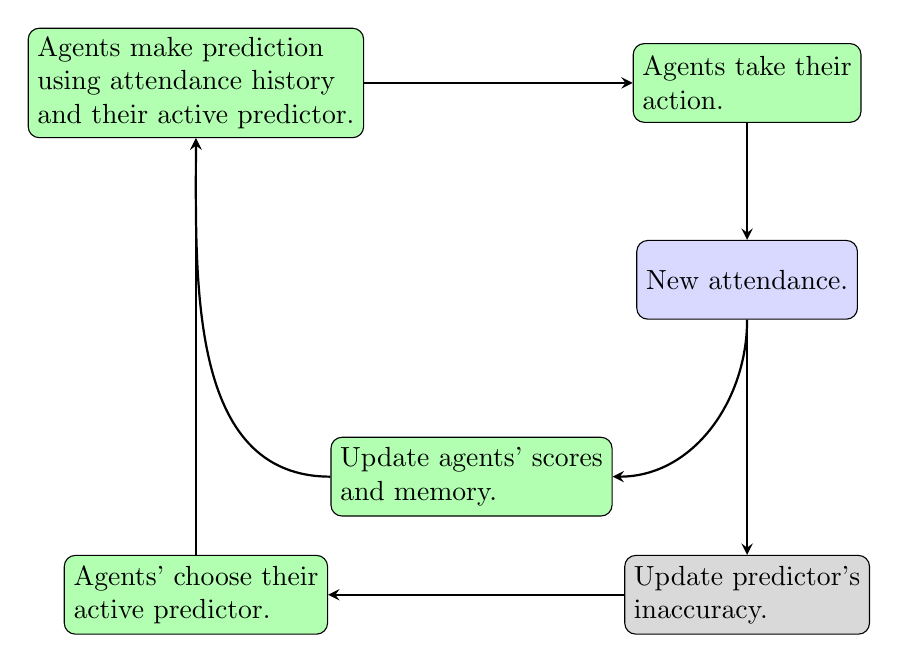
\begin{tikzpicture}
    \node[agente, align=left] (A) at (-1,2) {Agents make prediction\\ using attendance history\\ and their active predictor.};
    \node[agente, align=left] (B) at (6,2) {Agents take their\\ action.};
    \node[entorno, align=left] (C) at (6,-0.5) {New attendance.};
    \node[agente, align=left] (D) at (2.5,-3) {Update agents' scores\\ and memory.};
    \node[memoria, align=left] (E) at (6,-4.5) {Update predictor's\\ inaccuracy.};
    \node[agente, align=left] (F) at (-1,-4.5) {Agents' choose their\\ active predictor.};

    \draw[arrow] (A) edge [out=0, in=180, anchor=south] (B);
    \draw[arrow] (B) edge [out=270, in=90, anchor=south] (C);
    \draw[arrow] (C) edge [out=270, in=0, anchor=south] (D);
    \draw[arrow] (C) edge [out=270, in=90, anchor=south] (E);
    \draw[arrow] (D) edge [out=180, in=270, anchor=south] (A);
    \draw[arrow] (E) edge [out=180, in=0, anchor=south] (F);
    \draw[arrow] (F) edge [out=90, in=270, anchor=south] (A);
    
    %% \node[agente, align=left] (A) at (0,2) {Agent $i$:\\Softmax \\decision};
    %% \node[entorno, align=left] (B) at (5,2) {Bar:\\Consolidate $\bm{s}$};
    %% \node[entorno, align=left] (C) at (5,0) {Bar:\\Compute $A$};
    %% \node[entorno, align=left] (D) at (5,-2) {Bar:\\Compute\\ $\textsc{payoff}(a^i, A)$};
    %% \node[memoria, align=left] (E) at (0,0) {Agent $i$:\\Information\\level};
    %% \node[modelo, align=left] (F) at (-4,0.5) {Agent $i$:\\Update\\preferences};
    %% \draw[arrow] (A) edge [out=30, in=150, anchor=south] node {$a_i$} (B);
    %% %\draw[arrow] (A) edge [anchor=east] node {$a_i$} (E);
    %% \draw[line] (B) -- (C);
    %% \draw[line] (C) -- (D);
    %% \draw[arrow] (B) edge [out=180, in=30, anchor=north] node {$\bm{s}$} (E);
    %% \draw[arrow] (D) edge [out=180, in=-60, anchor=north] node {$\textsc{payoff}(a_i, A)$} (F);
    %% \draw[line] (F) edge [out=90, in=180, anchor=south] node {action preferences} (A);
    %% \draw[arrow] (E) edge [out=180, in=0, anchor=north] node {$\mathcal{S}$} (F);
  \end{tikzpicture}
\end{frame}

\end{document}
